
%(BEGIN_QUESTION)
% Copyright 2011, Tony R. Kuphaldt, released under the Creative Commons Attribution License (v 1.0)
% This means you may do almost anything with this work of mine, so long as you give me proper credit

Large electric motors are often equipped with some form of {\it soft-start} control, which applies power gradually instead of all at once (as in {\it ``across the line''} starting).  Here is an example of a simple ``reduced voltage start'' control system using a time-delay relay (TD1):

$$\includegraphics[width=15.5cm]{i02382x01.eps}$$

Analyze this ladder logic diagram, and explain the function of the time-delay relay, particularly how to interpret its switch symbol (with arrowhead).

\vfil

\underbar{file i02382}
\eject
%(END_QUESTION)





%(BEGIN_ANSWER)

This is a graded question -- no answers or hints given!
 
%(END_ANSWER)





%(BEGIN_NOTES)

In this system, resistors limit the motor's line current during the initial start-up period, and then are bypassed after the time delay relay times out.  

\vskip 10pt

Remember that time-delay relay symbols always use an arrowhead at the switch contact to denote the {\it direction of timing}.  With this switch, the arrowhead points in the closed direction, which means the relay takes time to close.  Being normally-open, this means the delay happens upon energization of the relay coil, the implication being that the relay will return to its normal (open) state immediately upon de-energization.

%INDEX% Electronics review: time-delay relay

%(END_NOTES)


